\section{Results}

\paragraph{Active panel.} The reconciled active MMLU panel is the 39-model HELM wide matrix with
14,042 scored items and zero missingness. The panel-validity gate passes with ability spread
0.580. Historical three-model files are provenance only, not the active panel.

\begin{figure}[t]
  \centering
  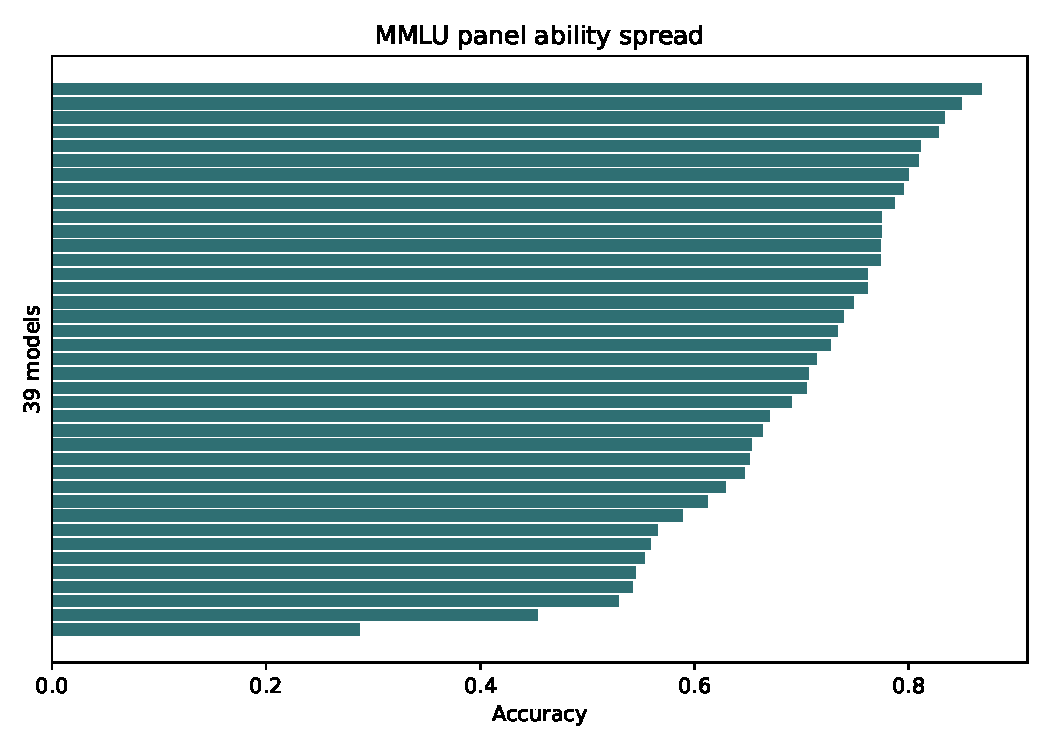
\includegraphics[width=0.78\linewidth]{figures/panel_ability_spread.pdf}
  \caption{Model accuracy spread across the active 39-model HELM MMLU panel.}
\end{figure}

\paragraph{Proxy psychometrics.} Proxy IRT diagnostics were computed for all 14,042 items. The
proxy run flags 1,037 negative-discrimination items, 1,342 near-zero-discrimination items, and
2,676 extreme-difficulty items. Rasch/1PL is not available for this wide matrix under the local BFGS
implementation, and the 2PL run exports proxy slopes only.

\begin{figure}[t]
  \centering
  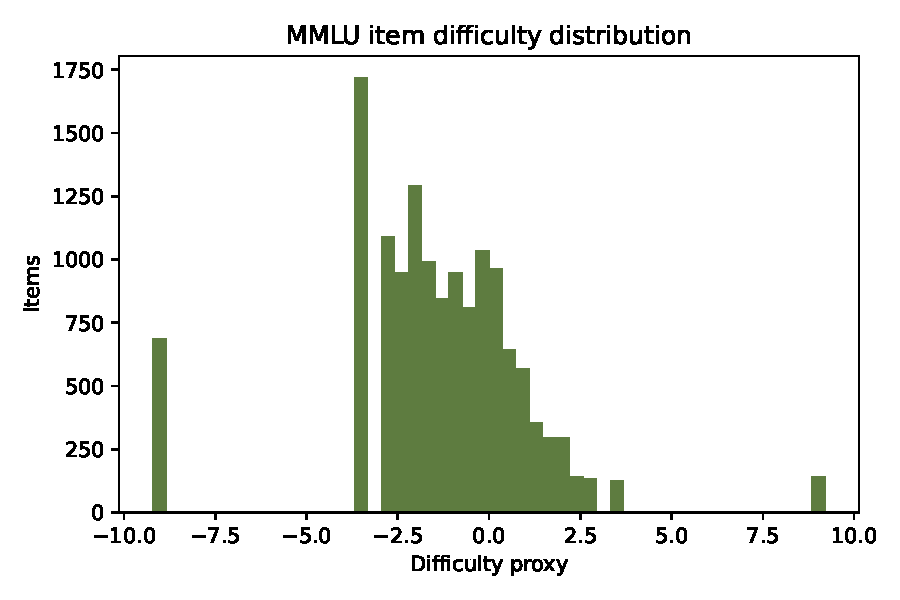
\includegraphics[width=0.48\linewidth]{figures/mmlu_item_difficulty_distribution.pdf}
  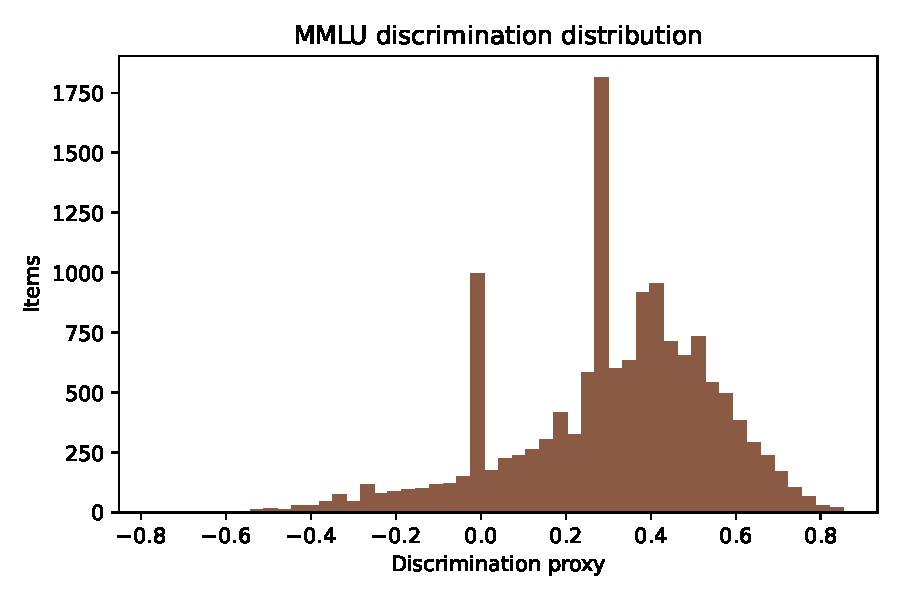
\includegraphics[width=0.48\linewidth]{figures/mmlu_discrimination_distribution.pdf}
  \caption{Proxy item difficulty and discrimination distributions on the active MMLU panel.}
\end{figure}

\paragraph{Ranking sensitivity.} Subject-level ranks vary substantially: every model has subject
rank range at least 3, and the maximum subject rank range is 30. In contrast, proxy
diagnostic-weighted ranking is very close to accuracy ranking, with Spearman correlation 0.998 and
maximum absolute rank delta 2.

\begin{figure}[t]
  \centering
  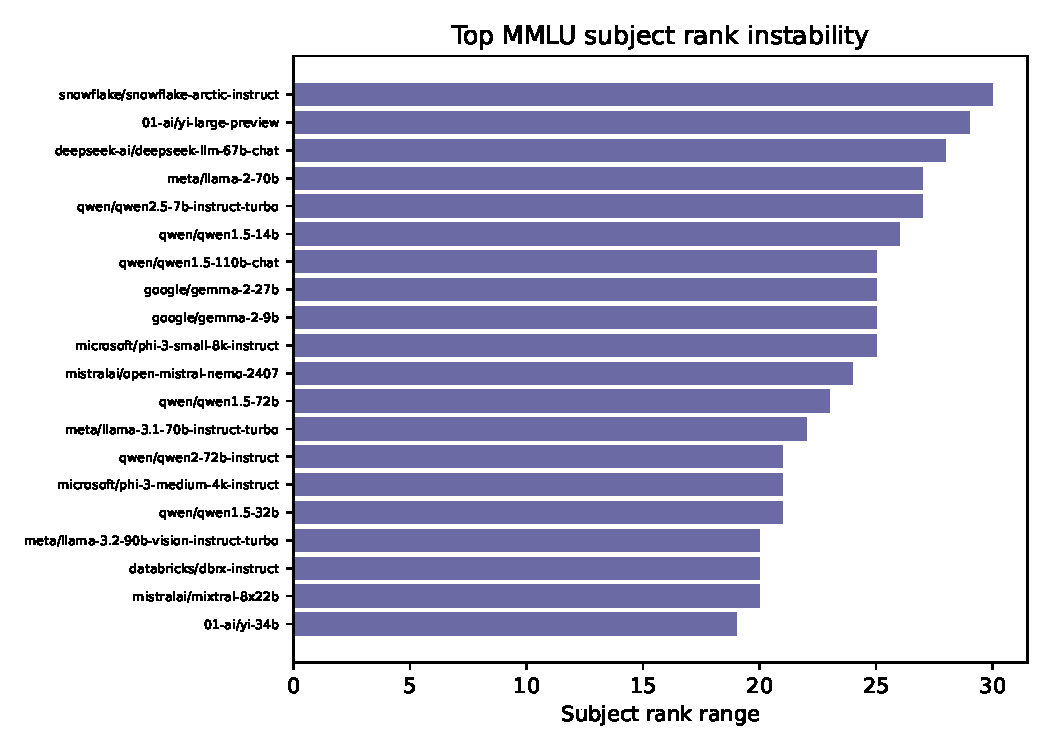
\includegraphics[width=0.48\linewidth]{figures/mmlu_ranking_instability.pdf}
  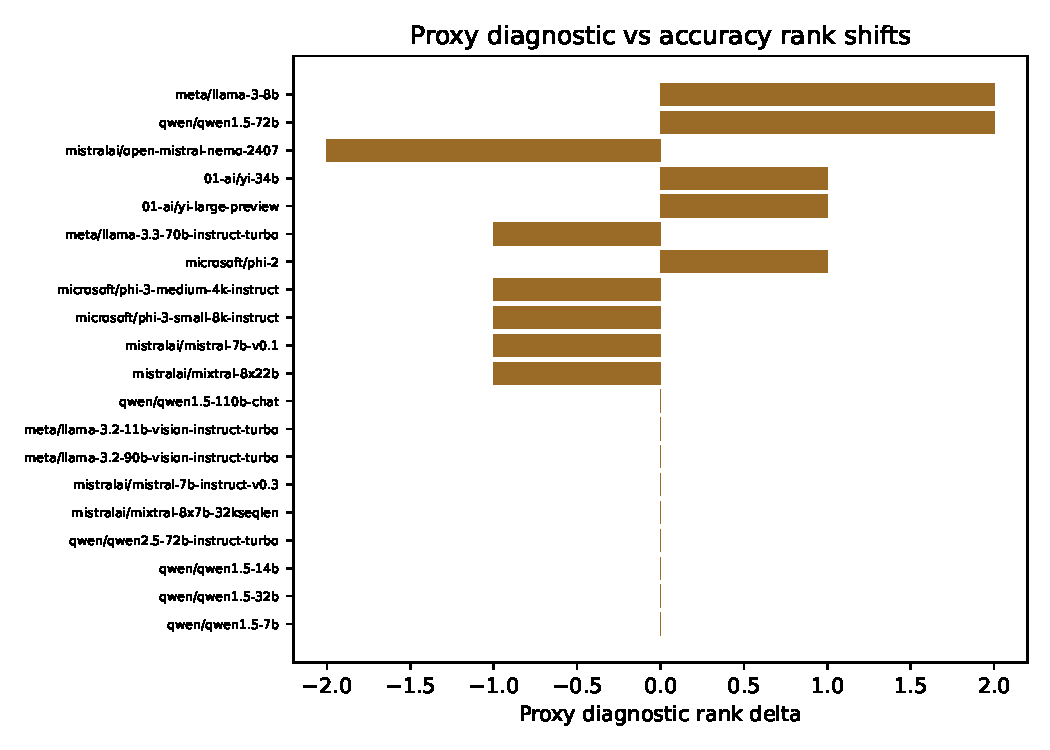
\includegraphics[width=0.48\linewidth]{figures/mmlu_diagnostic_disagreement.pdf}
  \caption{Subject-level rank instability is larger than proxy diagnostic-vs-accuracy rank shifts in this run.}
\end{figure}

\paragraph{Baselines.} Random-item and subject-stratified bootstrap baselines are stable at the top
of the ranking. Across 1,000 iterations per baseline, top-1 match rate is 1.0 and the 95th
percentile max absolute rank delta is 3.0.

\paragraph{MMLU-Redux.} Direct/hash alignment remains blocked: the current files have zero direct
item-id matches and no stable metadata or hash match path. The available structural alignment maps
370 labels by \texttt{subject\_numeric\_index}. Existing structural metrics remain weak/negative
(AUROC 0.539, AUPRC 0.0289, precision@10 0.0), so detection-success claims are blocked.

\paragraph{Deferred evidence.} Decoupled synthetic validation, second-benchmark evidence, Kaggle
output import, full Rasch/1PL, and full parametric 2PL remain \texttt{RESULT\_REQUIRED}.

\begin{table}[t]
  \centering
  \begin{tabular}{lrrl}
    \toprule
    Analysis & Spearman & Max rank delta & Claim state \\
    \midrule
    Proxy diagnostic vs. accuracy & 0.998 & 2 & proxy only \\
    Subject instability & -- & 30 & subject sensitivity \\
    \bottomrule
  \end{tabular}
  \caption{Ranking sensitivity summary. Proxy diagnostic weighting is close to accuracy ranking; subject ranks vary more.}
\end{table}
